\chapter{Methodology}\label{C:method} 

\section{Selecting Languages}
The languages explored in this study include Java, C\#, JavaScript and Lua. These languages were were selected because they each have large enough open source communities to gather meaningful corpora of projects and, between them, they offer a wide range of native object inheritance model implementations. They also provide a helpful division between two languages with native support for classical inheritance object models and two languages with native support for delegation object models.
\newline

Java and C\# both offer native implementations of classical inheritance so can be used to analyse the frequency of use of patterns which surround this classical inheritance model. These languages also allow an analysis of patterns which would behave differently under a delegation object model, representing cases which could be difficult to reimplement in another language with different native support.
\newline

JavaScript and Lua both offer delegation natively so can provide a measure of how often developers are making use of these delegation features. They also show how often developers in these languages are choosing to ignore the languages' native features in favour of classical inheritance models.

\section{Assembling Corpora}
To analyse the use of each language, we first needed to collect a corpus representative of that language's use in real world software development projects. In the case of Java, we adopted The Qualitas Corpus, which is a large collection of open source projects written in the Java language~\cite{QualitasCorpus}. Likewise, with JavaScript, we have adopted an existing corpus used by the team that developed JSClassFinder~\cite{JSClassFinder}.
\newline

For Lua and C\#, quality existing corpora could not be found so we had to build our own. For each of these languages, the top 25 open source projects were sourced from GitHub's ``Trending this month" list as of June, 2016. This source was chosen because it provides a group of projects for each language which are in active development as measured by GitHub, and which are easy to access. This helps to ensure that the analysis performed will contain repositories which are currently active so likely make use of newer language features.

\section{Static Analysis Tools}
The core of this empirical study is the analysis of corpora of code written in each of the investigated languages. This analysis makes use of many static code analysis methods including the following:
\begin{itemize}
	\item \texttt{grep} is used to perform regular expression searches on files. This can detect some of the more simple patterns explored in this paper. More specifically, an implementation of \texttt{grep} known as PCREGrep (Perl Compatible Regular Expression \texttt{grep}) was used to allow multiline analysis which is a requirement of a source code corpus analysis.
	\item ANTLR (Another Tool For Language Recognition) is a tool which accepts a language grammar as input and produces a lexer and parser. This lexer and parser can then accept a file which conforms to the grammar definition and construct a syntax tree to represent that file.
	\item JSClassFinder is a tool which detects patterns indicative of class and method declarations in JavaScript projects. It accepts JSON representations of the syntax trees of JavaScript files as input and produces the Class Usage Ratio of the syntax tree as its output~\cite{JSClassFinder}.
	\item Esprima accepts a JavaScript code file as input and produces a JSON representation of the syntax tree of that file as output. This JSON file can then be used as the input to the JSClassFinder tool.
\end{itemize}

\section{Java Analysis}
Finding occurrences of classical inheritance in Java is as simple as looking for the extends keyword with a \texttt{grep} regular expression search. Finding examples of delegation and forwarding is more difficult and requires more information about the syntax tree of the program. To achieve this, each program of the corpus was passed through ANTLR which parses each file according to a lexer and parser generated from a Java grammar. ANTLR then constructs an abstract syntax tree which can then be traversed to search for relevant patterns.
\newline

The process for analysing a Java project follows a pipeline structure where each file is parsed and analysed in isolation. The resulting statistics of each file are then aggregated to form the overall statistics across the projects. This file isolation is important because the syntax trees produced by ANTLR consume large amounts of memory so it is not possible to hold all the Java files for a project in memory simultaneously.
\newline

\begin{center}
	\captionof{figure}{Java Analysis Pipeline}
	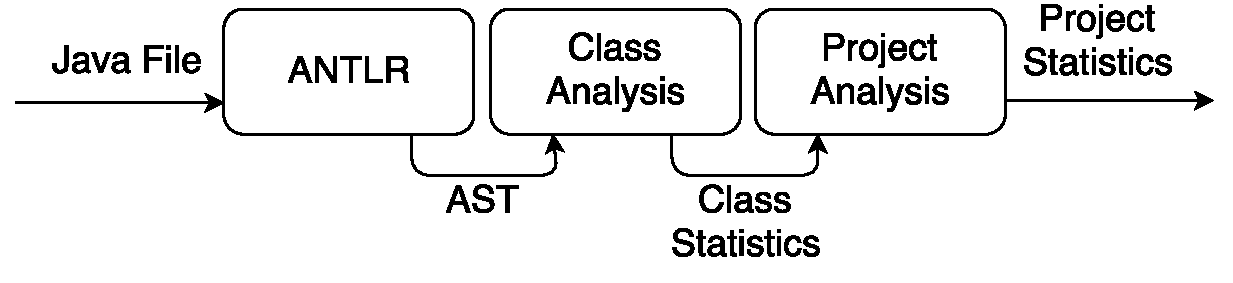
\includegraphics[scale=0.70]{AntlrPipeline.pdf}
\end{center}

\section{C\# Analysis}
As with Java, C\# was analysed using a lexer and parser generated by loading a C\# 6 grammar into ANTLR. The analysis for each project in the corpus was performed in three major passes:
\begin{enumerate}
	\item Use ANTLR, along with a C\# preprocessor grammar, to perform the first stage towards forming a syntax tree. This stage evaluates preprocessor directives in the program to ensure the remaining file can be transformed into a well formed syntax tree. Included in this stage is the removal of \cs{\#region} tags and conditional directives which exclude and include blocks of source code based on boolean arguments.
	\item Use ANTLR, along with a C\# program grammar, to create a syntax tree for each C\# code file in the corpus and traverse it to find all class declaration subtrees. Collect these class declarations to be explored in later steps.
	\item Run a visitor down each class declaration subtree, searching for all the methods and recording their modifiers. A type hierarchy is also established at this step to allow classes to find information about method calls they make which may be dispatched to a method in their superclass.
	\item Run another visitor down each class declaration tree and find constructors and check which methods are called against the modifiers found in the previous pass to determine which methods could miss their intended target under a different object initialisation model.
\end{enumerate}
The statistics gathered for each file in each project were then aggregated across the corpus to collect information about the corpus as a whole.

\subsection{Outliers}
The Mono project in the C\# corpus had to be modified to allow the project to be analysed successfully due to technical constraints. As the Mono project sets out to provide an open source implementation of the necessary components of a C\# compiler, it contained a copy of the entire .NET core library. This library was over 500MB in size so, after conversion to syntax trees through ANTLR, could not be reasonably analysed within 16GB of ram. For this reason, and because none of the other projects in this study or in \cite{QualitasCorpus} included copies of the source of their libraries, the .NET core library was removed from the Mono project. Every project across the corpora studied will have some dependency on a library, even if it is just the languages core libraries, so removing a copy of these libraries from Mono will ensure its comparability with the rest of the analysed data.
\newline

An interesting outlier file was found during the C\# analysis carried out in this study. A file titled \code{T\_1247520.cs} is defined in the Roslyn compiler project and is used in testing scenarios. This file contains 10,020 class definitions, each with no superclass, no subclasses, and no method or constructor definitions. The file is found in a \code{Test} directory so the assumption is that it is used as a compiler stress test. This file has been left in the corpus for the results found in Table \ref{CsResults} because I believe removing it would be making the disingenuous claim that all the file in the other corpora had been investigated to ensure they had no similar outliers. Despite this, it is interesting to see the changes to results when these class definitions are removed, thereby reducing the number of classes found by 10,020 but leaving the remaining counts unchanged.
\begin{itemize}
	\item The percentage of classes which extend another class increases from 26.87\% to 31.24\%.
	\item The percentage of classes which are extended by another class increases from 12.66\% to 14.72\%.
	\item The percentage of classes which make calls from local methods from a constructor increases from 2.47\% to 2.87\%.
	\item The percentage of classes with calls to local virtual, override, and abstract methods from their constructors increases proportionately with the change in all calls to local methods from constructors.
\end{itemize}

\section{JavaScript Analysis}
In JavaScript, there are many ways developers make use of classical inheritance patterns despite the lack of native support in the language. This is largely a result of the numerous libraries which offer their own implementation of classical inheritance behaviour. Some examples of these patterns can be found in the following table:
\begin{center}
	\captionof{table}{JavaScript Patterns}
	\begin{tabular}{|p{5cm}|p{9cm}|}
		\hline
		\multicolumn{2}{|c|}{JavaScript}                                                                                                                                                                  \\ \hline
		Inheritance 1                  & \code{var a = function( b )\{    c.call ( this , d );\}}                                                                                      \\ \hline
		Inheritance 2                  & \code{function Bar( x , y )\{    Foo.call ( this , x ) ;\}}                                                                                 \\ \hline
		Inheritance 3                  & \code{Foo.prototype = object.create ( Bar.prototype )}                                                                                      \\ \hline
		Inheritance 4 - Node.js        & \code{var className = defineClass(...)}                                                                                                           \\ \hline
		Inheritance 5 - Node.js        & \code{ util.inherits(...)}                                                                                                                         \\ \hline
	\end{tabular}\newline\newline
\end{center}

As a result of the wide ranging methods of implementing classical inheritance in JavaScript, the effort required to do so accurately is great. Prior work in the field made the JavaScript analysis in this study possible, primarily the existence of tool JSClassFinder~\cite{JSClassFinder}. The JavaScript analysis in this study consisted mainly of a recreation of the JSClassFinder study. JSClassFinder is a tool created by a team of researchers to analyse the extent to which JavaScript developers use classes in their projects.

\section{Lua Analysis}
The Lua corpus was analysed with \texttt{grep} to identify code patterns and keywords associated with class usage. There exists a variety of patterns used to implement classical inheritance in Lua as described by the Lua-Users Wiki~\cite{LuaObjectOrientation}. The analysis in this study attempts to uncover the proportion of the Lua corpus which is making use of object oriented paradigms and, to achieve this, analyses the code of each file to detect the particular patterns found in the object orientation tutorial.
\newline

The first of these patterns is the presence of \code{identifier = setmetatable()} in a Lua program. The \code{setmetatable()} function is the core of all suggested object orientation implementations so the detection of this pattern is vital. Unfortunately, while the use of this function is typically considered necessary for object orientation to exist in a Lua program, the pattern is often encapsulated in a function of a different name which makes the actual extent of object orientation usage more difficult to measure. In response to the practice of encapsulation of these patterns, this study has also included measures of the presence of two function names which are typically used to wrap these classical inheritance behaviours. These are the \code{class()} and \code{new()} functions.

\section{Java and C\# Metrics}
\subsection{Shared Metrics}
The first few metrics used in the analysis of Java and C\# match in order to develop an understanding of the differences in inheritance use between the languages.
\begin{enumerate}
	\item \textbf{Projects} measures the total number of individual projects in the corpus. This number is relevant because it allows us to determine the average size of projects in each corpus, which could possibly influence the results.
	\item \textbf{Classes} is the total count of class declarations in the corpus. This value acts as the basis for many of the other metrics, allowing values to be expressed as percentages of all classes.
	\item \textbf{Extending Classes} is a measure of the number of class definitions which include a reference to a superclass. This helps to determine the magnitude of inheritance usage in each language and also to find which classes could be impacted by changes to the object inheritance model.
	\item \textbf{Extended Classes} shows the number of class definitions which are referenced as a superclass by some other class definition. This value is important because many of the constructor patterns which are explored in this study only pose potential issues when a class is extended. This value is used to determine the percentage of classes which could have unexpected initialisation behaviour under a different object inheritance model.
\end{enumerate}

\subsection{Java Metrics}
In addition to these common metrics, we have some additional metrics which are specific to each language. The Java analysis focussed on the use of delegation and forwarding, an indication of a developer desire for those inheritance models. Additionally, the Java analysis investigated the prevalence of constructor patterns which would prevent projects being easily rewritten under a different object inheritance model. These are measured through the following metrics:
\begin{enumerate}
	\item \textbf{Classes with delegation} is a simple measure of classes containing the delegation patterns described in Section \ref{sec:delegation}
	\item \textbf{Classes with forwarding} is a simple count of the classes which contain the forwarding patterns described in Section \ref{sec:forwarding}
	\item \textbf{Classes with forwarding that extend another class} is the intersection between the previously mentioned \textbf{Classes with forwarding} and \textbf{Extended Classes} metrics.
	\item \textbf{Classes with local method calls in constructors} shows the number of classes which make a call to a local method from a constructor. This indicates an invocation which could be dispatched to an uninitialised object if the class were extended and the method overridden.
	\item \textbf{Classes storing this in constructors} shows the number of classes where the self reference of instances was found to be passed out from a constructor. This can occur as a field assignment or as a method parameter. This can present issues under models without Uniform Identity because other models do not always guarantee the self reference will remain the same after initialisation has completed.
	\item \textbf{Classes with local method calls or storing this in constructors} is a simple union of the two previous metrics, presenting a measure of all classes which could have constructor issues under another object inheritance model.
	\item \textbf{Extended classes with local method calls in constructors} is an intersection between the \textbf{Classes with local method calls in constructors} and \textbf{Extended Classes} metrics. This is important because local method calls in constructors can only be dispatched to an uninitialised subclass if a subclass exists.
	\item \textbf{Extended classes storing this in constructors} is an intersection between the \textbf{Classes storing this in constructors} and \textbf{Extended Classes} metrics. Under delegation, references passed out of the constructor from the most derived type in a hierarchy will behave as expected. For this reason, classes storing this in a constructor and which have a more derived type are of primary concern.
\end{enumerate}

\subsection{C\# Metrics}
C\# was analysed to provide a clearer understanding of the nature of local method calls made from constructors. The aim was to determine what proportion of those calls were dynamically dispatched and, therefore, could be invoked on a subclass when a call is made from a superclass. This is determined through a few important metrics:
\begin{enumerate}
	\item \textbf{Methods} is a count of all method definitions in the corpus. This is used as a baseline for determining the proportions of methods which exhibit certain properties.
	
	\item \textbf{Virtual Methods} measures the number of methods which are declared with a virtual modifier. This modifier is required to allow a method to be overridden by subclasses.
	
	\item \textbf{Override Methods} is a measure of the number of methods definitions which contain an override modifier. This means that the method has overridden some method on a superclass.
	
	\item \textbf{Classes with calls to local methods in constructors} is the number of classes which make a call to a local method from one or more of their constructors. This indicates an invocation which could be dispatched to an uninitialised object if the class were extended and the method overridden.
	
	\item \textbf{Classes with calls to local virtual methods in constructors} is the number of the local method calls from constructors where a matching method definition was found which contained a virtual modifier.
	
	\item \textbf{Classes with calls to local override methods in constructors} is the number of the local method calls from constructors where a matching method definition was found which contained an override modifier. This also implies the method was declared as virtual somewhere further up the hierarchy.
	
	\item \textbf{Classes with calls to local abstract methods in constructors} measures the same value as the previous two metrics, but matches against abstract modifiers. This is equivalent to a virtual definition except that the method \textit{must} be overridden by subclasses.
	
	\item \textbf{Classes with calls to methods that could not be found in constructors} measures the potential inaccuracy of the previous three metrics. This is discussed in detail in Section \ref{MethodNotFound}.
		
	\item \textbf{Delegates} is a measure of the prevalence of delegate usage in C\# projects. This was included because delegates relate to delegation but the numbers were very low so it was not investigated further.
\end{enumerate}

\section{JavaScript Metrics}
The JavaScript portion of this study is a reproduction of \textit{Does JavaScript Software Embrace Classes} by Silva et al~\cite{JSClassFinder}. The important metric drawn from this tool is the Class Usage Ratio (CUR) which measures the proportion of functions in a JavaScript project which exhibit class or method behaviour. The tool and this metric are described in more detail in Section \ref{sec:litJavaScript}.

\section{Lua Metrics}


\section{Evaluation}
The accuracy of the results of this study can be measured in terms of false positives against true positives and false negatives against true negatives. These can each be measured in different ways, but the process of testing for false positives is easier and more reliable than testing false negatives.

\subsection{False Positives}
\label{falsePositives}
False positives occur when the algorithms used to detect patterns in the corpora claim to have found an instance of that pattern, but the code does not match the definition exactly. Detecting false positives in the data can be achieved by investigating the results returned as matches against the patterns in the analysis to determine whether the are, in fact, exhibiting the behaviour for which the pattern is searching. In cases where the algorithms used to detect the patterns could be modified to ignore the false positives, they were. Despite this, there were some cases remaining where the search algorithms could not be easily fixed. Examples of these are as follows.
\begin{itemize}
	\item False positives may be returned for extendedness when the interface naming assumption explained in section \ref{interfaceNaming} fails and an interface is named in a way that makes it indistinguishable from a class.
	\item False positives may be returned for extendedness when the unique class name assumption explained in section \ref{uniqueNames} fails as classes may be considered extended when another class of the identical name is extended.
	\item False positives for delegation can occur when developers use code patterns which look identical to those of delegation but are modelling different intents. This is explained in more detail in section \ref{DetectingDelegation}.
\end{itemize} 

\subsection{False Negatives}
False negatives occur when the algorithms overlook code segments in the corpora which fulfil the criteria to be defined as an instance of the patterns under investigation. Examples of these cases are as follows.
\begin{itemize}
	\item There is room for false negatives in the C\# statistics on calls to local methods from constructors. The accuracy of this data is limited by the problem of inaccessible external code and the \cs{using static} pattern as explained in section \ref{MethodNotFound}. This is reflected in the final row of the table which measures the number of calls from constructors where the receiver of the call either could not be found or was another form of method call which was indistinguishable from a local method call.
	\item False negatives for subclassing in C\# can exist if a class is defined with a name which fulfils the requirements of the naming convention for interfaces as discussed in section \ref{interfaceNaming}.
\end{itemize}





